\chapter{FAHP多维资源建模和参数自动求解}
在上一章MRWS调度算法的评分函数中,根据资源的重要程度使用系数$\alpha_{i}(i=1,2,3,4,5), \quad\alpha_{1}+\alpha_{2}+\alpha_{3}+\alpha_{4}+\alpha_{5}=1$作为节点CPU、内存、磁盘I/O、网络带宽和已部署Pod数量的重要程度系数。本章需要对筛选后的节点和容器应用资源进行建模,并利用FAHP方法进行Pod应用多维权重参数的自动求解。

\section{模糊层次分析法FAHP}
模糊层次分析法FAHP~\cite{Kwong2002A,Hong2013Cloud}(Fuzzy Analytical Hierarchy Process)是在层次分析法的基础发展而来,常用于解决实际问题中影响决策问题的多种因素的权重。下面从层次分析法开始介绍,为弥补层次分析法的不足引入FAHP方法,然后举例说明如何使用该方法解决实际问题。

\subsection{FAHP方法介绍}
在许多实际问题中,通常有较多的解决方案,我们需要对影响方案的因素进行比较、判断、评价,然后做出选择,这种人为主观做出决策题的方式不但效率低下,结果也不够准确。层析分析法AHP~\cite{Saaty1994How,Deng2012}(Analytical Hierarchy Process)是由著名的美国运筹学家,匹茨堡大学的T.L.Saaty教授提出的一种层次权重决策分析方法。该方法用于解决复杂的多目标决策问题,将影响目标决策的因素分解为目标层、准则层和方案层等层次,使用数学方法对各因素权重进行精确求解。层次分析法将问题的总目标、各层子目标以及决策因素分解成多个层次结构,然后构建各层次的判断矩阵,求解判断矩阵的特征值。最大特征值对应的特征向量归一化获得上一层各元素对本层目标的优先权重,最后用加权和的方法递阶归并各备选方案对总目标的最终权重,选择权重最大的备选方案作为最终的目标。该方法是一个系统性的分析方法,先将问题分解成多个层次,然后对影响子目标的因素进行比较判断、最终进行综合决策。该方法结构层次清晰、单层的权重参数设置都会影响到最终的决策层,不断分割量化各因素的影响。层次分析法非常实用,将定量分析和定性分析相结合,用于解决许多实际问题如电力分配、旅游决策等,该方法计算简单明了,易于掌握。最后,该方法用于模拟人们解决问题的思维,所需的定量信息较少,仅需要对影响决策因素的重要性做出判断即可。

但是,层次分析法也具有较大的局限性,在一些场景下效果较差甚至无法使用。首先,该方法只能从实际的备选方案中帮助决策者选出较优的决策方案,不能给决策者提供新的解决方案或者反馈合理方案的意见,并且该方法是单目标决策方法,使用者只能从备选方案中选出一个较优的目标。其次,该方法模拟人类大脑决策过程,过于依赖于定性分析,只能进行粗略比较计算,不能完全做到精确模拟。最后,从层次结构转化为成对比矩阵过程中,判断者的主观因素影响过大,使用者不同,得出的最优方案也不尽相同,可重复性较差。并且随着影响决策因素的增加,构建的成对比矩阵阶数增大,计算难度和复杂度随之增加,很难一次性构建出满足一致性要求的成对比矩阵。

为减少人为主观因素对决策结果的影响,模糊层析分析法FAHP在层次分析法的基础上增加人为判断的模糊性。层析分析是通过两两比较构建成对比判断矩阵,而FAHP通过两两比较构建模糊成对比矩阵,提升了层次分析法解决问题的可靠性。在进行问题判断或专家咨询时,通过获得的不是一个具体值,而是一个模糊数,如三值判断(最低可能值、最可能值和最大可能值)、二值区间(上界和下界)等。下面介绍模糊数集的概念,一个明确的集合表示如下:
\begin{equation}
\mu_{A}(x) = \left\{\begin{array}{l}
1, x\in A \\ [0.3cm]
0, x\notin A
\end{array}\right.
\end{equation}
在明确的集合中,$x\in A$时值为1,$x\notin A$时值为0。但对于一个模糊数集,并不能完全明确x是否属于A,只能用[0,1]表示其隶属度。
\begin{equation}
\mu_{A}(x):U\to[0,1]
\end{equation}
\begin{math}\mu_{A}(x)\end{math}表示\begin{math}x\in A\end{math}的隶属度,也称\begin{math}\mu_{A}(x)\end{math}为集合A的隶属函数。对于任意的模糊数集,都对应一个隶属函数,隶属函数通常模仿概率论中的分布函数如正态分布、梯形分布、K次抛物线分布、S分布以及柯西分布等,值域在[0,1]上。

1983年,荷兰学者Van Loargoven首次提出用三角模糊数~\cite{Wang2010Triangular,Chou2003The}作为模糊数集的判断标准,并运用三角模糊数的运算和对数最小二乘法获取权重值。设论域R上的模糊数$\widetilde{M}$为三角模糊数,其对应的隶属函数\begin{math}\mu_{\widetilde{M}:}R\to[0,1]\end{math}满足下列函数:
\begin{equation}
\mu_{\widetilde{M}}(x) = \left\{\begin{array}{l}
0 \quad x<a \\ [0.2cm]
\frac{x-a}{b-a} \quad a\le x\le b \\ [0.2cm]
\frac{c-x}{c-b} \quad b\le x\le c \\ [0.2cm]
0 \quad x>c
\end{array}\right.
\end{equation}
$\widetilde{M}=(a,b,c) \quad a\le b\le c$,
a和c分别表示三角模糊数的上界和下界,b是隶属度为1的中间值,x=b时表示x完全属于$\widetilde{M}$,x在a和c之外的不属于模糊数$\widetilde{M}$。定义一个置信度$\alpha$可以将三元组的模糊数$\widetilde{M}$化为一个$\alpha$割集的二元形式,从而构建$\alpha$割集矩阵,设定优化参数后将二元值的矩阵转化成最终的判断矩阵。
\begin{equation}
	\widetilde{M}_{\alpha} = [l^{\alpha},u^{\alpha}]=[(b-a)\alpha+a,-(c-b)\alpha+c] \quad \forall \alpha\in[0,1]
\end{equation}
根据Arnold J. Kaufmann在文献~\inlinecite{Eastman1987Introduction}中的描述,$\alpha$割集后的基本运算规则如下:
\begin{equation}
\begin{split}
	\widetilde{M}_{\alpha} &= [m_{L}^{\alpha},m_{R}^{\alpha}] \\[0.2cm]
	\widetilde{N}_{\alpha} &= [n_{L}^{\alpha},n_{R}^{\alpha}] \\[0.2cm]
	\widetilde{M}_{\alpha}\oplus \widetilde{N}_{\alpha} &= [m_{L}^{\alpha}+n_{L}^{\alpha},m_{R}^{\alpha}+n_{R}^{\alpha}] \\[0.2cm]
	\widetilde{M}_{\alpha}\ominus \widetilde{N}_{\alpha} &= [m_{L}^{\alpha}-n_{L}^{\alpha},m_{R}^{\alpha}-n_{R}^{\alpha}] \\[0.2cm]
	\widetilde{M}_{\alpha}\otimes \widetilde{N}_{\alpha} &= [m_{L}^{\alpha}n_{L}^{\alpha},m_{R}^{\alpha}n_{R}^{\alpha}] \\[0.2cm]
	\widetilde{M}_{\alpha}\oslash \widetilde{N}_{\alpha} &= [m_{L}^{\alpha}/n_{L}^{\alpha},m_{R}^{\alpha}/n_{R}^{\alpha}] \\[0.2cm]
	\end{split}
\end{equation}
本文采用三角模糊数作为FAHP的隶属函数进行权重参数求解,并将三元组的$\widetilde{M}$=(a,b,c)转化成$\alpha$割集形式
$\widetilde{M}_{\alpha} =[(b-a)\alpha+a,-(c-b)\alpha+c] \quad \forall \alpha\in[0,1]$。

\subsection{FAHP求解权重参数步骤}
介绍完层次分析方法和模糊层析分析方法以及模糊数的基本概念后,下面用三角模糊数作为模糊程度的衡量值,FAHP求解权重参数流程如下:
\begin{figure}[H] % use float package if you want it here
	\centering
	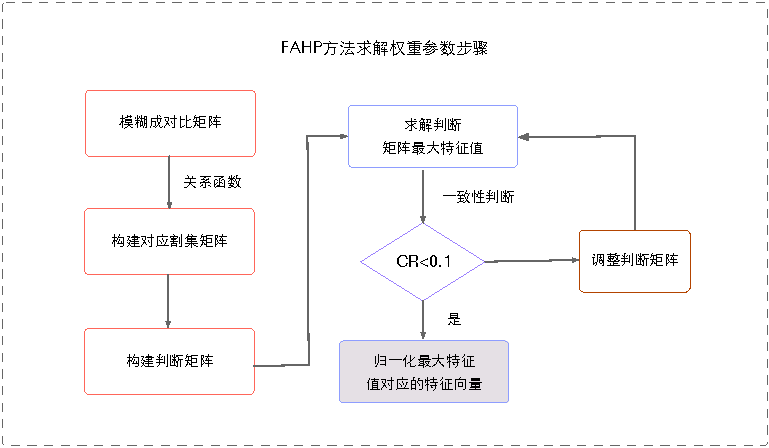
\includegraphics{fahp-flow}
	\caption{FAHP计算权重参数过程}
\end{figure}
如图4.2所示,使用FAHP方法计算权重参数的步骤可以分为构建模糊成对比矩阵、设置$\alpha$转化为$\alpha$割集矩阵、设置优化参数转化为判断矩阵,求解判断矩阵的最大特征值,检验判断矩阵是否满足一致性要求。若满足则将最大特征值对应的特征向量归一化作为权重参数值,否则需要调整判断矩阵值,重新进行特征值计算。下面详细介绍求解步骤:

1) 构建模糊成对比矩阵。在FAHP中,对影响决策因素进行两两对比并使用$\widetilde{1}\sim \widetilde{9}$表示其相对重要程度,值越大,表示该因素相对另一个因素对决策目标的影响越大,重要性越高。模糊数、相对重要程度、$\widetilde{M}$三元组及其$\alpha$割集如表4.1所示,可以构建最终的模糊成对比矩阵$\widetilde{A} $,其中的元素$\widetilde{a}_{ij} $表示因素i相对j的重要程度,模糊成对比矩阵中元素值如式(4-6)所示。
\begin{equation}
\widetilde{a}_{ij} = \left\{\begin{array}{l}
1 \quad i=j \\ [0.2cm]
\widetilde{1},\widetilde{3},\widetilde{5},\widetilde{7},\widetilde{9}\ or\ \widetilde{1}^{-1},\widetilde{3}^{-1},\widetilde{5}^{-1},\widetilde{7}^{-1},\widetilde{9}^{-1} \quad i\not=j  
\end{array}\right.
\end{equation}
\begin{table}[htbp]
	\centering\dawu[1.3]
	\caption{模糊数、相对重要程度和$\alpha$割集关系表}
	\begin{tabular}{|c|c|c|c|c|c|} \hline
		模糊数 & $\widetilde{1}$ & $\widetilde{3}$ & $\widetilde{5}$  & $\widetilde{7}$ & $\widetilde{9}$ \\ \hline
		重要性 & 同等重要 & 稍微重要 & 重要 & 明显重要 & 非常重要 \\ \hline 
		$\widetilde{M}$ & (1,1,3) & (1,3,5) & (3,5,7) & (5,7,9) & (7,9,11) \\ \hline 
		$\widetilde{M}_{\alpha}$ & [1,3-2$\alpha$] & [1+2$\alpha$,5-2$\alpha$] & [3+2$\alpha$,7-2$\alpha$] & [5+2$\alpha$,9-2$\alpha$] & [7+2$\alpha$,11-2$\alpha$]\\ \hline 
	\end{tabular}
\end{table}

2) 构建$\alpha$割集矩阵并转化为判断矩阵。构建模糊成对比矩阵后,根据表4.1将模糊数转化成三元组的三角模糊数,给定$\alpha$后,将三元组转化成$\alpha$割集$\widetilde{M}_{\alpha}=[l_{\alpha},u_{\alpha}]$,从而构建一个$\alpha$割集矩阵$\widetilde{A}_{\alpha}$,割集矩阵中的元素$\widetilde{a}_{ij}^{\alpha}$如式(4-7)所示。给定一个优化参数表示判断优化程度,可以将二元组的割集矩阵转化成判断矩阵方阵A,然后进行判断矩阵特征值和特征向量的求解。设给定的优化参数$\mu\in[0,1]$,将割集矩阵中上下界范围转化成判断矩阵的单值,判断矩阵中的元素$a_{ij}=(1-\mu)l_{\alpha}+\mu u_{\alpha}$,如式(4-8)所示。通过给定$\alpha$获得二元组的割集矩阵,给定割集矩阵一个优化参数$\mu$可以得到最终的判断矩阵A。
\begin{equation}
\widetilde{a}_{ij}^{\alpha} = \left\{\begin{array}{l}
1 \quad \widetilde{a}_{ij}=1 \\ [0.2cm]
[l_{\alpha},u_{\alpha}] \quad \widetilde{a}_{ij}\in{\widetilde{1},\widetilde{3},\widetilde{5},\widetilde{7},\widetilde{9}} \\ [0.2cm]
[\frac{1}{u_{\alpha}},\frac{1}{l_{\alpha}}] \quad \widetilde{a}_{ij}\in{\widetilde{1}^{-1},\widetilde{3}^{-1},\widetilde{5}^{-1},\widetilde{7}^{-1},\widetilde{9}^{-1}}
\end{array}\right.
\end{equation}
\begin{equation}
a_{ij} = \left\{\begin{array}{l}
1 \quad \widetilde{a}_{ij}=1 \\ [0.2cm]
(1-\mu)l_{\alpha}+\mu u_{\alpha} \quad \widetilde{a}_{ij}\in{\widetilde{1},\widetilde{3},\widetilde{5},\widetilde{7},\widetilde{9}} \\ [0.2cm]
\frac{1-\mu}{u_{\alpha}}+\frac{\mu}{l_{\alpha}} \quad \widetilde{a}_{ij}\in{\widetilde{1}^{-1},\widetilde{3}^{-1},\widetilde{5}^{-1},\widetilde{7}^{-1},\widetilde{9}^{-1}}
\end{array}\right.
\end{equation}

3) 计算判断矩阵最大特征值和特征向量。对判断矩阵特征值的求解是一个纯数学问题,求解方阵特征值和特征向量的方法有几何平均法(方根法)、算术平均平均法(和法)、最小二乘法(幂法)和特征向量法。几种方法求解的特征值近似相等,但也存在细微的差别,这种细微的误差可能会影响实际生产。通常情况下,几何平均法和算术平均获得的结果精确度较差,最小二乘法计算复杂度较高,因此使用特征向量法对判断矩阵的特征值和特征向量进行求解。在本文中,直接使用Python中numpy库eig()函数求解判断矩阵的特征值和特征向量。

4) 一致性检验和归一化权重。通过特征向量法获得判断矩阵的最大特征值$\lambda_{max}$及其对应的特征向量$\nu_{max}$后,需要进行层次单排序和层次总排序的一致性检验,用于检测特征向量和真实权值的契合度,即求解的权重值是否合理。判断矩阵一致性检测方法公式如式(4-9)所示。
\begin{equation}
\begin{split}
CI &= \frac{\lambda_{max}-n}{n-1} \\
CR &= \frac{CI}{RI}
\end{split}
\end{equation}
其中,$\lambda_{max}$是判断矩阵最大特征值,n是影响决策因素的数量即判断矩阵的阶数,CI表示一般一致性指标,RI是随机一致性指标,因此CR是随机一致性比率。若CR<0.1则判断矩阵满足一致性要求,否则需要调整判断矩阵直至其满足一致性判断要求。当CR<0.1时将$\lambda_{max}$对应的特征向量$\nu_{max}$归一化,其值w就是所需求解的权重值。常用的随机一致性指标RI的值如表4.2所示。
\begin{table}[htbp]
	\centering\dawu[1.3]
	\caption{随机一致性指标RI值}
	\begin{tabular}{|p{0.8cm}<{\centering}|p{0.8cm}<{\centering}|p{0.8cm}<{\centering}|p{0.8cm}<{\centering}|p{0.8cm}<{\centering}|p{0.8cm}<{\centering}|p{0.8cm}<{\centering}|p{0.8cm}<{\centering}|p{0.8cm}<{\centering}|p{0.8cm}<{\centering}|p{0.8cm}<{\centering}|} \hline
	n & 1 & 2 & 3 & 4 & 5 & 6 & 7 & 8 & 9 & 10 \\ \hline
	RI & 0 & 0 & 0.58 & 0.90 & 1.12 & 1.24 & 1.32 & 1.41 & 1.45 & 1.49 \\ \hline
	\end{tabular}
\end{table}

以上是用FAHP方法求解权重参数的全部过程,首先对影响决策的因素进行两两比较,构建模糊成对比矩阵,用$\widetilde{1}\sim \widetilde{9}$表示相对重要程度。针对模糊成对比矩阵,给定$\alpha\in[0,1]$获得割集矩阵,设定优化参数$\mu \in[0,1]$获得判断矩阵,计算判断矩阵的最大特征值和对应的特征向量,检测最大特征值是否满足随机一致性比率要求,最后将最大特征向量归一化获得权重值。

\subsection{FAHP求解权重参数示例}
上一小节介绍了FAHP求解权重参数的详细流程和计算方法,下面通过一个简单的例子展示该方法求解权重参数的计算过程。假设在一个物理问题中力学指数的评价由巴氏硬度、耐荷重性、耐冲击性和满水变形四个因素决定,其影响力学指数的判断因素层次如图4.2所示。
\begin{figure}[H] % use float package if you want it here
	\centering
	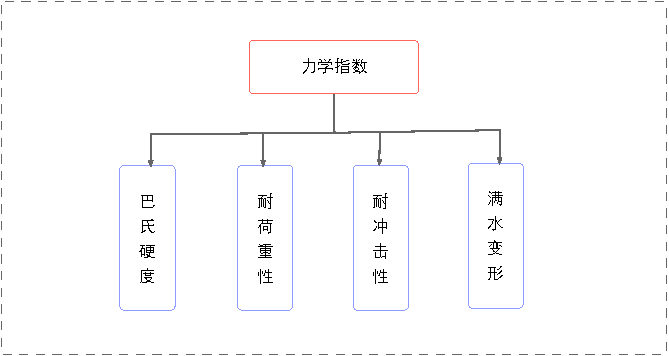
\includegraphics{fahp-example}
	\caption{力学指数的评价因素}
\end{figure}
某专家通过对影响力学指数的因素进行两两对比后给出其三角模糊判断数,根据其给出的模糊数构建模糊成对比矩阵如式(4-10),从左至右依次为巴氏硬度、耐荷重性、耐冲击性和满水变形。
\begin{equation}
\widetilde{A} = \left\{\begin{array}{cccc}
1 & \widetilde{3} & \widetilde{7} & \widetilde{5}  \\
\widetilde{3}^{-1} & 1 & \widetilde{5} & \widetilde{3} \\
\widetilde{7}^{-1} & \widetilde{5}^{-1} & 1 & \widetilde{3}^{-1} \\
\widetilde{5}^{-1} & \widetilde{3}^{-1} & \widetilde{3} & 1 \\
\end{array}\right\}
\end{equation}
给定$\alpha=0.5$和优化参数$\mu=0.5$,根据式(4-7)和(4-8)可以获得割集矩阵和判断矩阵,判断矩阵A如下:
\begin{equation}
A = \left\{\begin{array}{cccc}
1 & 3 & 7 & 5 \\
\frac{3}{8} & 1 & 5 & 3 \\
\frac{7}{48} & \frac{5}{24} & 1 & \frac{3}{8} \\
\frac{5}{24} & \frac{3}{8} & 3 & 1 \\
\end{array}\right\}
\end{equation}

使用特征向量法对判断矩阵进行特征值和特征向量求解,最大特征值$\lambda_{max}=4.21154$,其对应的特征向量值$\nu_{max}=[0.88297,0.41986,0.08951,0.18992]$,使用最大特征值对判断矩阵A的一致性进行判断,CR=0.082<0.1满足一致性要求。对其最大特征值对应的特征向量进行归一化,其权重w=[0.558,0.265,0.057,0.120]分别表示巴氏硬度、耐荷重性、耐冲击性和满水变形四个因素对力学系数影响的权重系数,用于对后面的目标层做出决策。

\section{容器应用多维资源权重自动求解}
上一小节详细介绍了FAHP方法求解权重系数的流程,并用一个力学系数的例子展示其计算过程。在MRWS调度算法中,需要使用容器应用各维资源的权重参数进行节点评分,由于需要调度的容器应用数量庞大,不能人为的给每一个容器应用的资源需求赋一个权重值,这样既不准确也不显示。因此,下面将介绍使用FAHP方法对容器应用的多维资源进行建模并自动求解。
\subsection{容器应用多维资源建模}
在MRWS调度算法中,集群中节点CPU、内存、磁盘和网络带宽以及已部署的Pod数量作为影响容器应用调度决策的因素,预选阶段筛选后的节点作为其调度的备选节点。不同的用户和应用场景对资源需求不同,容器云中允许用户配置应用的资源量既能节约成本,又能实现按需服务。首先对影响调度的因素进行分层建模,如图4.3所示,整个层次可以分为目标层、准则层和方案层。目标层是选择一个预选阶段过滤的后的节点作为容器应用调度的目标;准测层是影响调度决策的因素,包括节点CPU、内存、磁盘、网络带宽以及已部署Pod数量;方案层是所有满足容器资源需求的主机。从该层次模型中可以发现,每一个因素都对方案层直接施加影响,是一个全层次的模型结构。

调度算法的速度是衡量服务的重要指标,一种快速的调度算法对容器云至关重要。MRWS调度算法在优化的调度流程中,增加一个应用类型和对应的系数存储模块,初始可以通过数据中心感知的应用类型,分级建立部分权重系数库。一旦有新的容器应用请求,将资源需求和库中的资源层级进行对比,如果资源差值在可接受范围内,直接使用库中应用的系数作为待调度容器的权重参数,实现快速调度。若系数库中不存在该类型应用,需要重新计算该类应用的资源权重系数,并保存到系数库中,不断扩充应用参数库,也可以人工调整参数,提升精确度。在本文的方法中,权重参数根据容器应用资源需求与单位资源组的比值实现自动求解,无需用户给出模糊成对比矩阵,用户也可以对系数库加以修正。
\begin{figure}[H] % use float package if you want it here
	\centering
	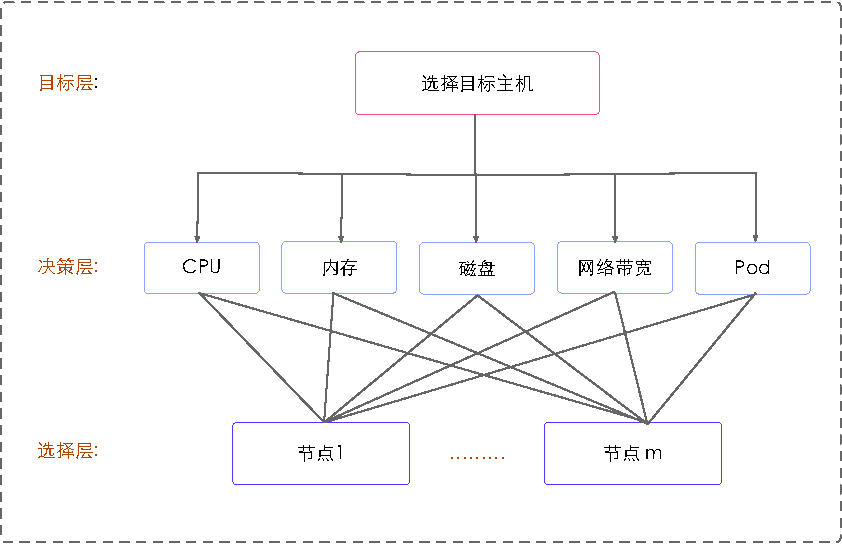
\includegraphics{fahp-model}
	\caption{多维资源递阶模糊层次结构}
\end{figure}
在云计算数据中心,CPU和内存一般是相对稀缺的资源,容器应用中CPU和内存相对其他资源需求重要性一般要高。单个节点上部署Pod数量较大,已部署Pod这个影响决策的因素相对其他因素的重要性较弱,但是大量小资源需求Pod会增加节点的管理成本。在构建模糊成对比矩阵时,该因素的模糊数较小,只是作为平衡各节点已部署Pod数量,容器应用的资源需求才是首要考虑因素。根据上述的层次结构图,下面介绍权重参数的自动求解方法。

\subsection{多维资源权重参数自动求解}
容器应用多维资源模糊层次结构如图4.3所示,大量容器应用进行模糊成对比矩阵构建时完全依赖人工判断既不准确也不适用于生产环境。在实际系统中,需要对每一个容器应用的多维资源进行权重参数求解,自动构建模糊成对比矩阵,然后转化为割集矩阵和判断矩阵,实现最大特征值的自动求解和判断矩阵的一致性检测。若判断矩阵不满足一致性要求,程序需要能自动调整判断矩阵直至其满足一致性检验。因此,如何对影响决策的CPU、内存、磁盘、网络带宽和已部署Pod等几个影响决策的因素构建模糊成对比矩阵成为解决问题的关键,整体的解决思路是用待调度容器资源需求占单位资源组的比例进行两两对比。设某个容器应用对各维度资源的需求和节点单位资源组如表4.3所示,需要求解容器应用各维度资源的权重系数$w_{c},w_{m},w_{d},w_{b},w_{p}$且$w_{c}+w_{m}+w_{d}+w_{b}+w_{p}=1$。
\begin{table}[htbp]
	\centering\dawu[1.3]
	\caption{某容器应用和节点单位资源组}
		\begin{tabular}{|p{1.5cm}<{\centering}|p{1.5cm}<{\centering}|p{1.5cm}<{\centering}|p{1.5cm}<{\centering}|p{1.8cm}<{\centering}|p{1.5cm}<{\centering}|} \hline
			Resources & CPU & Memory & Disk & Bandwidth & Pod \\ \hline
			U-Node & C & M & D & B & ..  \\ \hline
			Pod & $C_{0}$ & $M_{0}$ & $D_{0}$ & $B_{0}$ & 1  \\ \hline
			Weight & $w_{c}$ & $w_{m}$ & $w_{d}$ & $w_{b}$ & $w_{p}$ \\ \hline
		\end{tabular}
\end{table}

在构建模糊成对比矩阵时,根据容器应用资源需求和单位资源组的比值之间的差值确定模糊数。如在对比CPU和内存的重要性时,采用$|C_{0}/C-M_{0}/M|$作为判断依据,使用$\widetilde{1}\sim\widetilde{9}$表示相对重要程度的大小,在[0,1]范围内将其切分为5份,根据比值差值自动构建模糊数。模糊成对比矩阵的模糊数、容器应用各维度资源需求和单位资源组的比值差值对应如表4.4所示。在数据中心的集群中,各节点的资源构成通常是异构的,即单个服务器各维度资源不同,不能直接使用容器应用与各节点资源比值的差值获取模糊数,需要抽象出单位资源组概念作为构建依据。如1个core的CPU、1G内存、50G磁盘、10M带宽作为一个单位资源组,单位资源组的大小根据集群实际情况确定,将容器应用和单位资源组的比值差值作为模糊数的依据。最后使用表4.4的方法构建模糊成对比矩阵。
\begin{table}[htbp]
	\centering\dawu[1.3]
	\caption{模糊数和资源比值差值对应表}
	\begin{tabular}{|p{1.8cm}<{\centering}|p{1.8cm}<{\centering}|p{1.8cm}<{\centering}|p{1.8cm}<{\centering}|p{1.8cm}<{\centering}|p{1.8cm}<{\centering}|} \hline
		差值 & (0, 0.2] & (0.2, 0.4] & (0.4, 0.6] & (0.6, 0.8] & (0.8, 1) \\ \hline
		模糊数 & $\widetilde{1}$ & $\widetilde{3}$ & $\widetilde{5}$ & $\widetilde{7}$  & $\widetilde{9}$  \\ \hline
		差值 & (-0.2,0] & (-0.4, -0.2] & (-0.6, -0.4] & (-0.8, -0.6] & (-1, -0.8]  \\ \hline
		模糊数 & $\widetilde{1}^{-1}$ & $\widetilde{3}^{-1}$ & $\widetilde{5}^{-1}$ & $\widetilde{7}^{-1}$ & $\widetilde{9}^{-1}$  \\ \hline
	\end{tabular}
\end{table}

针对已部署Pod这一影响调度的因素,其重要性相对其他资源要低,容器应用对该资源的需求以及节点上能部署的Pod总数都无法度量,不能像其他资源一样直接通过比值的差值作为模糊数的获取依据。因此,将CPU、内存、磁盘和网络带宽四种资源的比值从小到大排序,相较于Pod这一因素的重要性依次获得模糊数为(${\widetilde{3},\widetilde{5},\widetilde{7},\widetilde{9}}$),反之,Pod相对于其他资源的模糊数为(${\widetilde{3}^{-1},\widetilde{5}^{-1},\widetilde{7}^{-1},\widetilde{9}^{-1}}$)。

容器应用资源需求和单位资源组比值的差值可以获取各因素之间两两对比的模糊数,从而构建模糊成对比矩阵,最终自动获取割集矩阵和判断矩阵。求解出判断矩阵的特征值和对应的特征向量,判断矩阵满足一致性判断后,归一化出各因素的权重值,实现权重参数的自动求解。下面用一个实际的例子详细展示模糊成对比矩阵的构建以及最终权重参数的求解过程。

若某个集群的单位资源组配置如表4.5所示,集群中各节点各维度资源的配置都是单位资源组的整数倍,单位资源组是构成集群资源的最小组成单元。提出单位资源组的概念主要是为解决异构集群的场景,通常数据中心的集群都是异构的,尤其是在云计算中心中,需要将互联网上大量闲置的计算机作为服务计算单元,这种整合的闲置资源,并不是同构服务集群。
\begin{table}[htbp]
	\centering\dawu[1.3]
	\caption{物理集群单位资源组配置}
	\begin{tabular}{|p{2cm}<{\centering}|p{2cm}<{\centering}|p{2cm}<{\centering}|p{2cm}<{\centering}|p{2cm}<{\centering}|} \hline
		类型 & CPU(M) & MEM(M) & Disk(G) & BW(M) \\ \hline
		数量 & 1200 & 8000 & 500 & 50  \\ \hline
	\end{tabular}
\end{table}

在该数据中心集群上进行应用容器的调度,设某个应用容器对各维度资源的需求和集群单位资源组的比值如表4.6所示。
\begin{table}[htbp]
	\centering\dawu[1.3]
	\caption{某应用容器的资源需求}
	\begin{tabular}{|p{1.8cm}<{\centering}|p{1.8cm}<{\centering}|p{1.8cm}<{\centering}|p{1.8cm}<{\centering}|p{1.8cm}<{\centering}|p{1.8cm}<{\centering}|} \hline
		类型 & CPU(M) & MEM(M) & Disk(G) & BW(M) & Pod \\ \hline
		数量 & 300 & 1100 & 210 & 40 & 1 \\ \hline
		占比 & 0.25 & 0.1375 & 0.42 & 0.8 & - \\ \hline
	\end{tabular}
\end{table}

根据各维度资源所占比值的差值作为模糊数的依据,可以构建出该容器应用的模糊成对比矩阵,已部署Pod因素影响较弱,其他因素与该因素对比获取的模糊数较大。自动构建的模糊成对比矩阵如式(4-12)所示,行和列依次为CPU、内存、磁盘、网络带宽以及已部署Pod等影响决策的因素,通过两两对比确定模糊数后获得一个5*5的模糊成对比方阵。
\begin{equation}
\widetilde{A} = \left\{\begin{array}{ccccc}
1 & \widetilde{1} & \widetilde{1}^{-1} & \widetilde{5}^{-1} & \widetilde{5}  \\
\widetilde{1}^{-1} & 1 & \widetilde{3}^{-1} & \widetilde{7}^{-1} & \widetilde{3} \\
\widetilde{1} & \widetilde{3} & 1 & \widetilde{3}^{-1} & \widetilde{7} \\
\widetilde{5} & \widetilde{7} & \widetilde{3} & 1 & \widetilde{9} \\
\widetilde{5}^{-1} & \widetilde{3}^{-1} & \widetilde{7}^{-1} & \widetilde{9}^{-1} & 1 \\
\end{array}\right\}
\end{equation}

给定割集参数$\alpha=0.5$,优化参数$\mu=0.5$,参数$\alpha$反映模糊数中最大可能值的模糊程度,即真实值与最大可能值的距离,当$\alpha=1$时,模糊数的真实值就是最大可能值,$\alpha=0$时模糊程度出现最大范围,真实值和最大可能值接近程度最低。$\mu$作为优化参数,在模糊给定$\alpha$后反映上界和下界的取值,$\mu=1$时取上界值,$\mu=0$时取下界值。两个参数对权重参数的影响可以参考文献[26],该文献对两个参数对权重产生的影响进行了详细的分析。将上述的模糊成对比矩阵转化为割集矩阵,然后再转变为实际判断矩阵如(4-13)所示。
\begin{equation}
A = \left\{\begin{array}{ccccc}
1 & \frac{3}{2} & \frac{3}{4} & \frac{5}{24} & 5 \\
\frac{3}{4} & 1 & \frac{3}{8} & \frac{7}{48} & 3 \\
\frac{3}{2} & 3 & 1 & \frac{3}{8} & 7 \\
5 & 7 & 3 & 1 & 9 \\
\frac{5}{24} & \frac{3}{8} & \frac{7}{48} & \frac{9}{80} & 1 \\
\end{array}\right\}
\end{equation}

使用特征向量法求解判断矩阵的特征值和对应的特征向量,获得的特征值$\lambda_{max}=5.2498$,计算一般一致性指标CI=(5.2498-5)/4=0.0623,查找随机一致性RI表在n=5时其值RI=1.12,因此随机一致性比率CR=CI/RI=0.0558<0.1,判断矩阵满足随机一致性比率CR<0.1的要求。

满足一致性的判断矩阵A最大特征值$\lambda_{max}$对应的特征向量$\nu_{max}$的值为(0.2291, 0.1452, 0.3607, 0.8903, 0.0600),将该特征向量归一化获得容器应用CPU、内存、磁盘、网络带宽以及已部署Pod几个因素的权重系数$w=(w_{c}, w_{m}, w_{d}, w_{b}, w_{p})=(0.136, 0.086, 0.214, 0.528, 0.036)$。从权重参数可以看出,该容器应用是一个网络密集型的应用,该应用对网络带宽资源需求更多,其权重参数最大,因此,权重参数也能反映容器应用对某个维度资源的需求量。至此,一个完整的自动构建模糊成对比矩阵并实现各维资源权重参数自动求解过程完成。

MRWS调度算法中,容器应用在进行调度时需要对集群中节点进行评分,选择评分最高的节点作为容器调度目标,在对节点空闲资源评分时需要使用容器应用需求资源权重系数作为乘积系数。在式(3-4)和(3-8)中,$\alpha$系数就是待调度容器应用各维资源的权重系数,该系数大小反映待调度容器对某个维度资源需求量。如一个CPU密集型应用,系数$\alpha_{1}$较大,节点中若某个节点CPU资源空闲较多,则该节点评分相对较高,Pod调度到该节点的几率就越大。使用FAHP对待调度容器Pod各维资源进行层次建模后,通过容器应用资源需求和集群单位资源组比值之间的差值构建模糊成对比矩阵,最终自动求解的各维资源权重值就是空闲资源评分系数。其中单位资源组大小、$\alpha$割集系数和优化参数$\mu$的选取对调度评分都至关重要。使用系数调节后的MRWS算法可以实现容器云集群中各维资源的均衡利用,将CPU密集型应用调度到CPU剩余资源较多并且各维资源使用较为平衡的节点上,其他密集型的应用调度相似。因此,这种调度方法将各种密集型容器应用尽可能分散混合部署到节点上,避免大量相同密集型集中调度到相同节点上,造成某一维度的资源资源不足,尤其是在大数据处理多维计算框架应用调度的场景下,能够提升集群资源利用率和负载均衡性,极大增强集群的服务性能。

\section{本章小结}
在MRWS调度算法中,需要求解容器应用各维度资源的权重参数作为节点评分乘积系数,本章应用FAHP求解容器应用各维资源权重参数。首先从层次分析法AHP开始,详细介绍该方法的历史背景和解决问题的能力。为减少专家判断的主观性和模糊性,使用各种分布函数作为模糊数,选定三角模糊数作为判断依据,从而引入了模糊层次分析法FAHP,并使用$\widetilde{1}\sim\widetilde{9}$表示因素之间相对重要程度。接着详细阐述应用该方法求解权重系数的步骤,构建模糊成对比矩阵,给定置信度$\alpha$将其转化为割集矩阵,设置优化参数$\mu$后转化为判断矩阵,求解判断矩阵最大特征值和特征向量,检测该判断矩阵是否满足一致性要求。通过调整判断矩阵,满足一致性判断要求后,归一化最大特征值对应的特征向量获得各维度资源的权重值,接着通过一个力学系数的例子展示各计算步骤的详细计算过程。

最后,使用FAHP求解容器应用各维度资源的权重参数,先对各资源需求和备选节点进行层次建模,获得一个全层次的模型结构。将容器应用各维度资源和单位资源组的比值之间的差值作为自动构建模糊成对比矩阵的依据,获得模糊成对比矩阵,并转化为割集矩阵和判断矩阵,实现权重参数的自动求解。使用一个具体的容器应用展示该应用各维度资源的权重系数自动计算过程,最终获得的权重参数就是MRWS调度算法中用于各节点空闲资源和资源平衡性的评分计算系数。








